\part{Library resources}
\frame{\partpage}

\begin{frame}{Library catalogue}
	\begin{center}
		\url{http://library.fxplus.ac.uk/}
	\end{center}
\end{frame}

\begin{frame}{Web proxy}
	Insert \texttt{.ezproxy.falmouth.ac.uk} at the end of the \textbf{domain name}
		(before the \texttt{/})
	\pause
	\begin{center}
		\texttt{http://www.example.com/example/page.html}
		
		\pause $\downarrow$
		
		\texttt{http://www.example.com\uline{.ezproxy.falmouth.ac.uk}/ example/page.html}
	\end{center}
\end{frame}

\begin{frame}{ACM Digital Library}
	\begin{center}
		\small\url{http://dl.acm.org.ezproxy.falmouth.ac.uk/}
	\end{center}
\end{frame}

\begin{frame}{IEEE Xplore}
	\begin{center}
		\small\url{http://ieeexplore.ieee.org.ezproxy.falmouth.ac.uk/}
	\end{center}
\end{frame}

\begin{frame}{GDC Vault}
	\begin{center}
		\small\url{http://www.gdcvault.com.ezproxy.falmouth.ac.uk/}
		
		\vspace{2ex}
		
		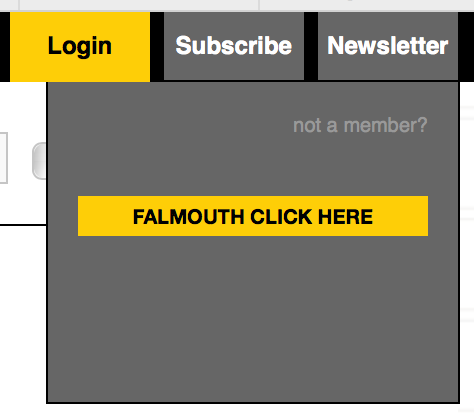
\includegraphics[width=0.4\textwidth]{gdc_login}
	\end{center}
\end{frame}

\begin{frame}{Ethics of paywalls}
	\begin{itemize}
		\pause\item Is it ethical for publishers to charge for access to publicly-funded academic research?
		\pause\item Many journals offer free \textbf{open access}
			\begin{itemize}
				\pause\item Some high quality, some low quality...
			\end{itemize}
		\pause\item Many authors put papers on their \textbf{personal websites}
			\begin{itemize}
				\pause\item Some publishers allow this, others turn a blind eye
			\end{itemize}
		\pause\item Sites like \textbf{sci-hub} aim to be a ``Pirate Bay for papers''
	\end{itemize}
\end{frame}
